%\documentstyle[epsf,twocolumn]{jarticle}       %LaTeX2e仕様
\documentclass[twocolumn]{jarticle}     %pLaTeX2e仕様(platex.exeの場合)
% \documentclass[onecolumn]{ujarticle}   %pLaTeX2e仕様(uplatex.exeの場合)
%%%%%%%%%%%%%%%%%%%%%%%%%%%%%%%%%%%%%%%%%%%%%%%%%%%%%%%%%%%%%%
%%
%%  基本バージョン
%%
%%%%%%%%%%%%%%%%%%%%%%%%%%%%%%%%%%%%%%%%%%%%%%%%%%%%%%%%%%%%%%%%
\setlength{\topmargin}{-45pt}
%\setlength{\oddsidemargin}{0cm}
\setlength{\oddsidemargin}{-7.5mm}
%\setlength{\evensidemargin}{0cm}
\setlength{\textheight}{24.1cm}
%setlength{\textheight}{25cm}
\setlength{\textwidth}{17.4cm}
%\setlength{\textwidth}{172mm}
\setlength{\columnsep}{11mm}

%\kanjiskip=.07zw plus.5pt minus.5pt


% 【節が変わるごとに (1.1)(1.2) … (2.1)(2.2) と数式番号をつけるとき】
%\makeatletter
%\renewcommand{\theequation}{%
%\thesection.\arabic{equation}} %\@addtoreset{equation}{section}
%\makeatother

%\renewcommand{\arraystretch}{0.95} 行間の設定
%%%%%%%%%%%%%%%%%%%%%%%%%%%%%%%%%%%%%%%%%%%%%%%%%%%%%%%%
%\usepackage{graphicx}   %pLaTeX2e仕様(\documentstyle ->\documentclass)
\usepackage[dvipdfmx]{graphicx}
\usepackage{subcaption}
\usepackage{multirow}
\usepackage{amsmath}
\usepackage{url}
\usepackage{ulem}
\usepackage{algorithm}
\usepackage{algorithmic}
\usepackage{listings} %,jlisting} %日本語のコメントアウトをする場合jlistingが必要
%ここからソースコードの表示に関する設定
\lstset{
  basicstyle={\ttfamily},
  identifierstyle={\small},
  commentstyle={\smallitshape},
  keywordstyle={\small\bfseries},
  ndkeywordstyle={\small},
  stringstyle={\small\ttfamily},
  frame={tb},
  breaklines=true,
  columns=[l]{fullflexible},
  numbers=left,
  xrightmargin=0zw,
  xleftmargin=3zw,
  numberstyle={\scriptsize},
  stepnumber=1,
  numbersep=1zw,
  lineskip=-0.5ex
}
%%%%%%%%%%%%%%%%%%%%%%%%%%%%%%%%%%%%%%%%%%%%%%%%%%%%%%%%
\begin{document}

	%bibtex用の設定
	%\bibliographystyle{ujarticle}

	\twocolumn[
		\noindent
		\hspace{1em}
		前期研究発表会資料 2022 年 7 月 6 日 (水)
		\hfill
	  M2 杉山 竜弥
		\vspace{2mm}

		\hrule
		\begin{center}
			{\Large \bf 手描きスケッチの類似度}
		\end{center}
		\hrule
		\vspace{9mm}
	]

\section{はじめに}

% TODOs

% 実験 2

% 原稿をパワポに変換
% まとめと結論

% 発表練習

% (要素技術)
% 原稿仕上げ
% みてもらう

% 休み

% 授業
% 発表練習

  近年,機械学習の発展を背景に人工知能 (Artificial Intelligence : AI) が注目を浴びている.
  AI は単純なパターン認識では人間の能力を凌駕する性能を示す一方で,人間の情緒や感性に関する分野,特に人間の創作物への AI の適用はいまだ困難である.
  創作物の中でも,スケッチは,年齢,国籍,文化にかかわらず,幅広く共感可能な表現であるため重要度が高い.
  このため,感性を取り扱う分野での重要な AI の課題の 1 つとされてきた.
  また人工知能で画像データを扱う問題の場合,
  画像データの形式は画素の集合で高次元なラスタ形式のことが一般に多く,
  次元が少なく描き順の情報も持てるベクター形式での研究は多くない.

  本研究ではベクター形式のイラストのスケッチデータを用いて,
  創作物の 1 つである絵描き歌の生成を目指す.
  絵描き歌は画像,言語,音楽など様々なモーダルを含むため,
  極めて創作性が高い創作物の形態である.
  先行研究では単純なスケッチに対して,
  オブジェクトと位置関係を示す文章の生成に成功している.
  本研究では先行研究の手法を改良しより複雑なスケッチについて,
  絵描き歌らしい情緒的な歌詞を生成することを目標とし,
  改良したスケッチ分割手法を提案する.


\section{要素技術}

  \subsection{Sketch-rnn}	\label{tau}
    sketch-rnn とは深層学習を用いて,人間がイラストを描くときの一連の描き順を学習することでユーザのイラストを補完,推測する深層学習を利用したモデルである.
    % 図 \ref{fig:one} に sketch-rnn の学習モデルを構成する Variational Autoencoder (VAE) \cite{NIPS2017_7011} を示す.
    sketch-rnn の学習モデルは Variational Autoencoder (VAE) を基に構成されている.
    入力はスケッチの時系列を含む描き順を意味する行列であり,潜在ベクトルがエンコーダの出力となる.
    また,デコーダの出力は入力と同じ,画像を生成できる行列となる.


	\subsection{描き順データ}
		Google が公開する描き順データセットである QuickDraw! \cite{Cheema:2012:QID:2207676.2208550} の形式を使用する.
		この形式では, 1 つの手描きスケッチを構成する描き順データは行列で保持される.
		描き順データの行方向は手描きスケッチの描き始めから描き終わりまでのペンの状態に関する情報を時系列に沿って保持する.
		また,描き順データの列方向はある時刻 $t$ におけるペンの状態を保持しており,$x$ 座標の相対値, $y$ 座標の相対値,ストロークの描き終わりのブール値をそれぞれベクトルで持っている.

    \subsection{cos類似度}
コサイン類似度は、そのまま、ベクトル同士の成す角度の近さを表現するため、三角関数の普通のコサインの通り、1に近ければ類似しており、0に近ければ似ていないことになる。

\begin{equation}
  \cos( \overrightarrow{a}, \overrightarrow{b} ) =
  \frac{\overrightarrow{a} \cdot \overrightarrow{b}}{|\overrightarrow{a}| |\overrightarrow{b}|}
\end{equation}

    \subsection{akaze}
類似画像検索は任意の画像に対して類似している画像
を探すことである. 本研究では, 類似画像検索のアルゴ
リズムとして Accelerated KAZE (AKAZE) \cite{alcantarilla2011fast} とヒス
トグラム比較を用いた. AKAZE は特徴点およびその特
徴量を抽出するアルゴリズムの一つであり, 拡大縮小や
回転に強いという利点がある. 本研究における類似度の
計算には特徴点マッチングをし, 距離の平均を取るとい
う手法を用いた. 特徴点マッチングでは距離を算出して
いるため同一画像の場合, 類似度は 0 となり, 値が小さ
くなるほど類似度が高いことを示す. ヒストグラムは横
軸を画素値, 縦軸を画素値の出現頻度と設定したグラフ
である. ヒストグラムから画像のコントラスト, 明るさ,
画素値の分布を確認することができる. ヒストグラム比
較では主に色を用いた類似画像検索が可能となっている.

\section{提案手法}

\subsection{絵描き歌}
絵描き歌生成システムについて,
藤井ら \cite{} の先行研究では,~であった.

この問題を「スケッチの類似度比較」「スケッチの分割」「クラスラベルから歌詞生成」の 3 つに分割した.

絵描き歌では,似ている別のスケッチを合成することでプログレッシブ?的に目的のスケッチを完成させる.
そこで目的のスケッチを「全体スケッチ」,元のスケッチの一部を取り出したものを「部分スケッチ」とし,
部分スケッチの和が全体スケッチとなるような分割方法を実験する.

まず「スケッチの類似度比較」では,
2 つのスケッチ同士の類似度を求める場合の適当な指標を定める.

次に「スケッチの分割」では,
求めた類似度指標によって最適な分割を求め,
歌詞生成のための情報として部分スケッチのクラスラベルを獲得する.

「クラスラベルから歌詞生成」では,
すでに得たクラスラベルやその位置情報から,
絵描き歌の歌詞を言語モデルを利用して生成する.

\subsection{手法}
本研究では絵描き歌生成のためにまず「スケッチの類似度比較」と「スケッチの分割」を実験した.
それぞれを実験 1,実験 2 とする.

実験 1 ではスケッチの類似度指標となる 3 つの候補について,
スケッチの類似度を比較しその結果を定性的に評価した.

実験 2 では実験 1 で求めた指標を用いて実際に部分スケッチを求め,結果を比較した.


\section{実験1}
% \subsection{目的}

\begin{figure*}[tb]
 \begin{minipage}{1\hsize}
 	\begin{center}
 		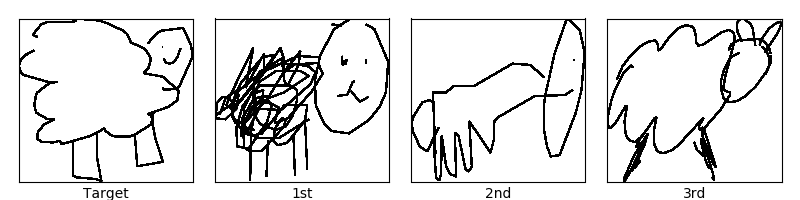
\includegraphics[clip,width=120mm]{sketch_trained_sim_A_0.png}
 		\caption{(手法A) Sketch RNN}
 		\label{fig:exp1_a}
 	\end{center}
 \end{minipage}

  \begin{minipage}{1\hsize}
  	\begin{center}
  		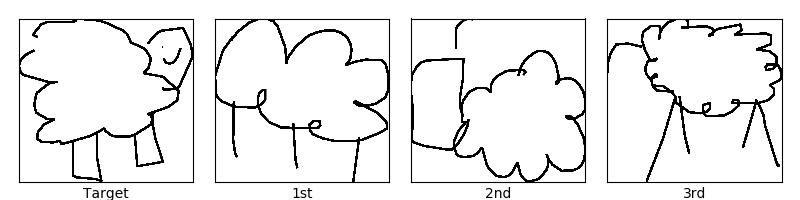
\includegraphics[clip,width=120mm]{sketch_trained_sim_B_0.png}
  		\caption{(手法B) AKAZE}
  		\label{fig:exp1_b}
  	\end{center}
  \end{minipage}

   \begin{minipage}{1\hsize}
   	\begin{center}
   		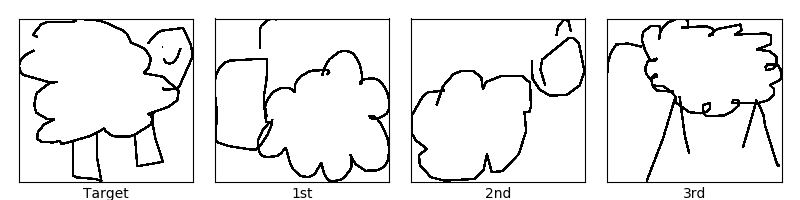
\includegraphics[clip,width=120mm]{sketch_trained_sim_D_0.png}
   		\caption{(手法C) Sketch RNN + AKAZE}
   		\label{fig:exp1_c}
   	\end{center}
   \end{minipage}
\end{figure*}

実験 1 では最適なスケッチの類似度指標を求める.
スケッチでは線を書く順番の「途中経過」と完成した「最終状態」を合わせた 2 つの状態があり,
この 2 つの状態を比較する必要がある.

途中経過はスケッチの時系列データを扱うことが出来る Sketch RNN を利用した.
Sketch RNN は Variational Autoencoder (VAE) であるため,
スケッチの時系列データを入力することで潜在ベクトル $z$ を得ることが出来る.
この $z$ のコサイン類似度を途中経過の類似度指標とした.

ここに数式

最終状態はスケッチを画像化し,画像比較手法 AKAZE で比較することにした.
先行研究では画質評価手法 Structural Similarity (SSIM) が用いられていたが,
AKAZE は特徴点マッチングをするため画像の内容を比較できる.

ここに数式

% y=\frac{\frac{\left(120-x\right)}{10}}{\left(1+\frac{\left(120-x\right)}{10}^{2}\right)^{0.5}}

これらを足し合わせ,途中経過と最終状態の両方を考慮する混合指標を

ここに数式

とし,式 ~ でスケッチの類似度指標を評価する.
時間の都合上~は 1 とした.

\subsection{実験設定}
スケッチデータセット QuickDraw から,対象とするスケッチとこれと比較するスケッチ 10 枚を取り出し,
3 つの類似度指標で実験した.
取り出したスケッチは全て "sheep" クラスで揃えた.

実験の設定は表 \ref{tab:setting1} に示す.
Sketch RNN のパラメータは事前に長時間学習したものを使用した.

\begin{table}[tb]
  \begin{center}
    \caption{実験1の設定}
    \begin{tabular}{|c|c|} \hline
       & name \\ \hline
      step & 150,000 \\ \hline
      class & 345 \\ \hline
      latent & (128, ) \\ \hline
      learning rate & 0.0000 \\ \hline
      learning rate & 0.0000 \\ \hline
      learning rate & 0.0000 \\ \hline
      learning rate & 0.0000 \\ \hline
      learning rate & 0.0000 \\ \hline
    \end{tabular}
    \label{tab:setting1}
  \end{center}
\end{table}

\subsection{結果}
% A[(7, 0.9862899), (6, 0.89415294), (2, 0.7782751), (1, 0.57062423), (8, 0.4869256), (0, 0.0013451368), (3, -0.21240741), (9, -0.21476299), (5, -0.5499855), (4, -0.9028328)]
% B[(8, -116.04807692307692), (1, -116.8173076923077), (5, -118.45192307692308), (3, -120.98076923076923), (9, -121.09615384615384), (2, -121.10576923076923), (4, -122.03846153846153), (0, -130.45192307692307), (6, -131.46153846153845), (7, -131.46153846153845)]
% = [(8, 0.3675329896053509), (1, 0.3032792943562569), (5, 0.15298536646415564), (3, -0.09760859402959103), (9, -0.10896271676452136), (2, -0.10990703386698913), (4, -0.1997384988151555), (0, -0.7225552339045035), (6, -0.7535157530723093), (7, -0.7535157530723093)]

% C[(8, 1.0934066387256818), (5, 0.9155709468131241), (1, 0.2629781539584698), (6, 0.228598204332781), (7, 0.17851659365315453), (2, -0.05635251758133125), (3, -0.9260878840381359), (9, -1.0704136511746165), (4, -1.1764581166587835), (0, -1.580862833925866)]
% D[(1, 1.511369831256345), (4, 1.341358246262741), (5, 0.5409496028127758), (8, -0.017384995408811332), (9, -0.06231150135711422), (3, -0.1333689828363287), (2, -0.16729802033620456), (6, -0.6606084867923497), (0, -0.831266857121777), (7, -0.8643148704974889)]


図 \ref{fig:exp1_a}, \ref{fig:exp1_b}, \ref{fig:exp1_c} に実験 1 の結果を示す.
左から対象のスケッチと類似度が高いと判断された上位 3 つのスケッチである.

Sketch RNN のみの場合は,描き順を考慮しているため最終状態はばらばらとなった.
しかし胴体と頭,足を持った羊が右を向いていることから,描き順という点で評価すると妥当であると言える.

次に AKAZE のみの場合は,羊毛の表現がなされているスケッチが選ばれており,
Sketch RNN ノミの場合と比較して極めて似ていることがわかる.
一方で体の部位や向きなどの描き順は無視されている.

最後に両方を混合した指標は,AKAZE のみの場合と大きな変化はないが
 2 番目のスケッチは片方のみの場合ではなかったスケッチで,
 羊毛と体の向きが類似しており 比較がうまくいく場合もあることが確認された.

AKAZE の影響が強いことと Sketch RNN の性能が高くないことから,
係数 $a$ を調整する必要がある.


\section{実験2: スケッチの分割}

\begin{figure*}[tb]

 \begin{minipage}{1\hsize}
 	\begin{center}
 		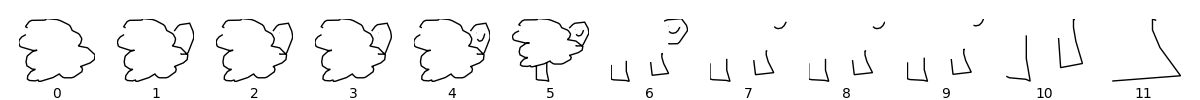
\includegraphics[clip,width=170mm]{origin.png}
 		\caption{分割候補となる部分スケッチ}
 		\label{fig:exp2_o}
 	\end{center}
 \end{minipage}
\vspace{2zh}

  \begin{minipage}{1\hsize}
  	\begin{center}
  		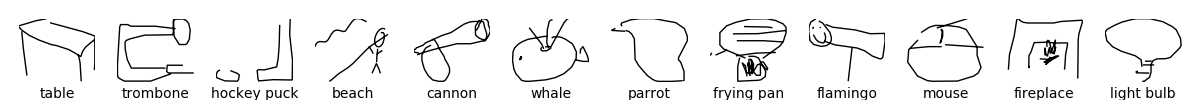
\includegraphics[clip,width=170mm]{sheep_a.png}
  		\caption{Sketch RNN の推定結果}
  		\label{fig:exp2_a}
  	\end{center}
  \end{minipage}
 \vspace{1.5zh}

   \begin{minipage}{1\hsize}
     \begin{center}
       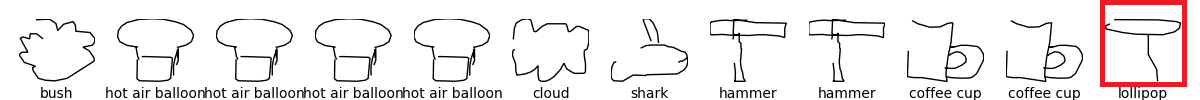
\includegraphics[clip,width=170mm]{sheep_b.png}
       \caption{AKAZE の推定結果}
       \label{fig:exp2_b}
     \end{center}
   \end{minipage}
  \vspace{1.5zh}

    \begin{minipage}{1\hsize}
      \begin{center}
        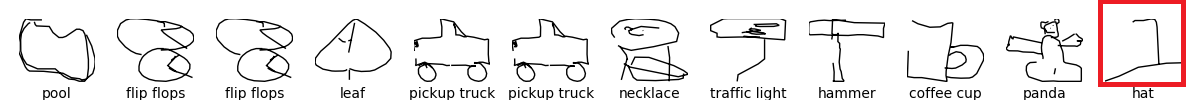
\includegraphics[clip,width=170mm]{sheep_c.png}
        \caption{Sketch RNN + AKAZE の推定結果}
        \label{fig:exp2_c}
      \end{center}
    \end{minipage}

    \vspace{1zh}

\end{figure*}




実験 2 では実験 1 で求めた指標を用いて実際に部分スケッチを求めた.

実験 1 の 3 つの類似指標それぞれで,
部分スケッチに最も近いデータベース中のクラスを求め,
対象のスケッチから最尤の部分スケッチを 1 つ分割した.

\subsection{設定}
分割方法はスケッチのストローク列の中で 1 箇所分割するように部分スケッチを得た.

データベースの 345 クラスの代表スケッチから
最も類似度の高いものを部分スケッチの推定クラスとし,
全体で最大の類似度となった分割を求める.

実験 1 同様に "Sheep" クラスを分割対象として選んだ.
このスケッチは 7 画であるため,候補は 12 個となった.

\subsection{結果}

図 \ref{fig:exp2_o} ~ \ref{fig:exp2_c} に実験 2 の推定結果を示す.
図 \ref{fig:exp2_o} はストローク列の 1 箇所で分割される可能性がある部分スケッチの候補である.
図 \ref{fig:exp2_a} ~ \ref{fig:exp2_c} は各類似度におけるそれぞれの推定する類似スケッチとなる.
図中の赤枠は類似度最大の部分スケッチである.

AKAZE 類似度を利用している手法の部分スケッチが一致した.
最も似ているのは Sketch RNN + AKAZE の"hat" クラスと思われる.
途中経過と最終状態を両方考慮することで,
類似度の性能が上がっている可能性がある.
定量的に評価するためアンケート調査を行いたい.

主観では体を "bush" や "cloud" ,足を "coffee cup" と比較してほしかったため,
単純な部分スケッチが選ばれにくいような補正が必要であると考えられる.

\section{まとめと今後の課題}
書き順を含むスケッチデータに対して~実験をし,類似度指標の考察をした.

絵描き歌用のデータセットを整備すること.

分割したクラスに対して言語モデルを通して,絵描き歌の歌詞を生成することが課題としてあげられる.

ここにテキストを入力してください.ここにテキストを入力してください.ここにテキストを入力してください.ここにテキストを入力してください.ここにテキストを入力してください.ここにテキストを入力してください.ここにテキストを入力してください.ここにテキストを入力してください.

% 参考文献リスト
\bibliographystyle{unsrt}
\bibliography{ref}
\end{document}
